\section{Results}
Results!

\begin{figure}[t]
\centering
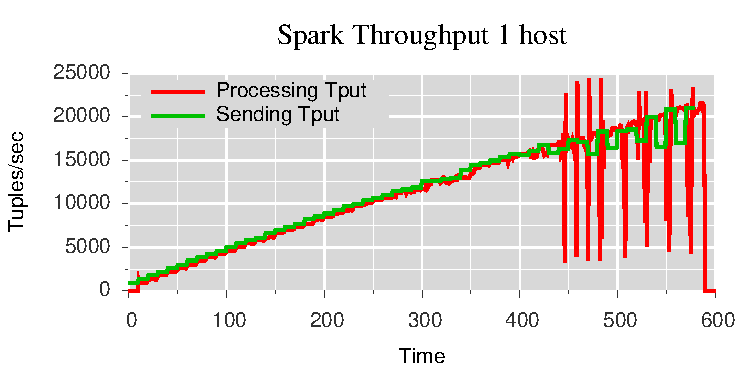
\includegraphics[width=1\linewidth]{figures/sp1_tput.pdf}
%\vspace{-0.3in}
\caption{Throughput/Time for a single Spark host. We sent 100B tuples at a
slowly ramped up rate from 1K tuples/sec to 30k tuples/sec with a step size of
500 tuples/sec. The sending rate remained constant for 10 seconds before
transitioning to the next throughput.}
\label{fig:sb1-tput}
\end{figure}

\begin{figure}[t]
\centering
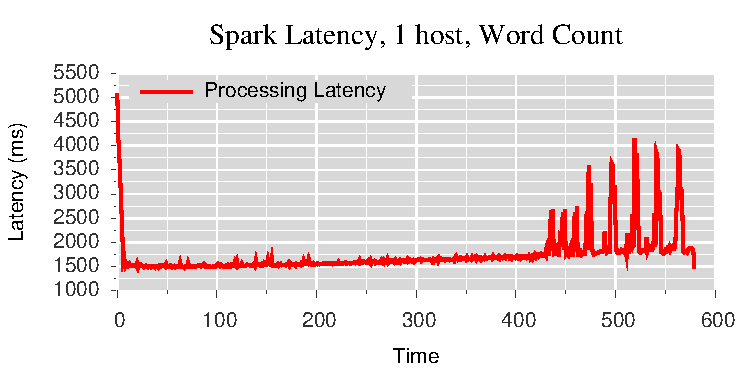
\includegraphics[width=1\linewidth]{figures/sp1_latency.pdf}
%\vspace{-0.3in}
\caption{Average latency to process tuples for a single Spark host. Similar to
Figure~\ref{fig:sb1-tput} we sent 100B tuples at a slowly ramped up rate from 1K
tuples/sec to 30k tuples/sec with a step size of 500 tuples/sec. The sending
rate remained constant for 10 seconds before transitioning to the next
throughput. The astute reader will notice that the latency spike in this graph
occurs at the same time as the loss in throughput consistency in
Figure~\ref{fig:sb1-tput}.}
\label{fig:label-me-if-you-want}
\end{figure}

